
\documentclass[journal,onecolumn]{IEEEtran}

\usepackage[utf8]{inputenc}
\usepackage{graphicx}
%\usepackage[spanish,activeacute]{babel}
%\usepackage[english,spanish]{babel}
%
% If IEEEtran.cls has not been installed into the LaTeX system files,
% manually specify the path to it like:
% \documentclass[journal]{../sty/IEEEtran}





% Some very useful LaTeX packages include:
% (uncomment the ones you want to load)


% *** MISC UTILITY PACKAGES ***
%
%\usepackage{ifpdf}
% Heiko Oberdiek's ifpdf.sty is very useful if you need conditional
% compilation based on whether the output is pdf or dvi.
% usage:
% \ifpdf
%   % pdf code
% \else
%   % dvi code
% \fi
% The latest version of ifpdf.sty can be obtained from:
% http://www.ctan.org/tex-archive/macros/latex/contrib/oberdiek/
% Also, note that IEEEtran.cls V1.7 and later provides a builtin
% \ifCLASSINFOpdf conditional that works the same way.
% When switching from latex to pdflatex and vice-versa, the compiler may
% have to be run twice to clear warning/error messages.






% *** CITATION PACKAGES ***
%
%\usepackage{cite}
% cite.sty was written by Donald Arseneau
% V1.6 and later of IEEEtran pre-defines the format of the cite.sty package
% \cite{} output to follow that of IEEE. Loading the cite package will
% result in citation numbers being automatically sorted and properly
% "compressed/ranged". e.g., [1], [9], [2], [7], [5], [6] without using
% cite.sty will become [1], [2], [5]--[7], [9] using cite.sty. cite.sty's
% \cite will automatically add leading space, if needed. Use cite.sty's
% noadjust option (cite.sty V3.8 and later) if you want to turn this off
% such as if a citation ever needs to be enclosed in parenthesis.
% cite.sty is already installed on most LaTeX systems. Be sure and use
% version 4.0 (2003-05-27) and later if using hyperref.sty. cite.sty does
% not currently provide for hyperlinked citations.
% The latest version can be obtained at:
% http://www.ctan.org/tex-archive/macros/latex/contrib/cite/
% The documentation is contained in the cite.sty file itself.






% *** GRAPHICS RELATED PACKAGES ***
%
\ifCLASSINFOpdf
  % \usepackage[pdftex]{graphicx}
  % declare the path(s) where your graphic files are
  % \graphicspath{{../pdf/}{../jpeg/}}
  % and their extensions so you won't have to specify these with
  % every instance of \includegraphics
  % \DeclareGraphicsExtensions{.pdf,.jpeg,.png}
\else
  % or other class option (dvipsone, dvipdf, if not using dvips). graphicx
  % will default to the driver specified in the system graphics.cfg if no
  % driver is specified.
  % \usepackage[dvips]{graphicx}
  % declare the path(s) where your graphic files are
  % \graphicspath{{../eps/}}
  % and their extensions so you won't have to specify these with
  % every instance of \includegraphics
  % \DeclareGraphicsExtensions{.eps}
\fi
% graphicx was written by David Carlisle and Sebastian Rahtz. It is
% required if you want graphics, photos, etc. graphicx.sty is already
% installed on most LaTeX systems. The latest version and documentation
% can be obtained at: 
% http://www.ctan.org/tex-archive/macros/latex/required/graphics/
% Another good source of documentation is "Using Imported Graphics in
% LaTeX2e" by Keith Reckdahl which can be found at:
% http://www.ctan.org/tex-archive/info/epslatex/
%
% latex, and pdflatex in dvi mode, support graphics in encapsulated
% postscript (.eps) format. pdflatex in pdf mode supports graphics
% in .pdf, .jpeg, .png and .mps (metapost) formats. Users should ensure
% that all non-photo figures use a vector format (.eps, .pdf, .mps) and
% not a bitmapped formats (.jpeg, .png). IEEE frowns on bitmapped formats
% which can result in "jaggedy"/blurry rendering of lines and letters as
% well as large increases in file sizes.
%
% You can find documentation about the pdfTeX application at:
% http://www.tug.org/applications/pdftex




% *** MATH PACKAGES ***
%
%\usepackage[cmex10]{amsmath}




% *** PDF, URL AND HYPERLINK PACKAGES ***
%
\usepackage{url}
% url.sty was written by Donald Arseneau. It provides better support for
% handling and breaking URLs. url.sty is already installed on most LaTeX
% systems. The latest version and documentation can be obtained at:
% http://www.ctan.org/tex-archive/macros/latex/contrib/url/
% Basically, \url{my_url_here}.




% *** Do not adjust lengths that control margins, column widths, etc. ***
% *** Do not use packages that alter fonts (such as pslatex).         ***
% There should be no need to do such things with IEEEtran.cls V1.6 and later.
% (Unless specifically asked to do so by the journal or conference you plan
% to submit to, of course. )

% correct bad hyphenation here
\hyphenation{op-tical net-works semi-conduc-tor}

\begin{document}
%
% paper title
% can use linebreaks \\ within to get better formatting as desired
% Do not put math or special symbols in the title.

\newcommand{\titlepaper}{Formato para la presentación de reportes a una Columna}

\title{\titlepaper}

\renewcommand\IEEEkeywordsname{Palabras clave}

% author names and affiliations
% transmag papers use the long conference author name format.

\author{\IEEEauthorblockN{Darío Ramsés Gutiérrez Rodríguez}

\IEEEauthorblockA{email: \url{ramsensei@estudiantec.cr}}
\IEEEauthorblockA{\\Área Académica Ingeniería en Computadores}
\IEEEauthorblockA{\\Instituto Tecnológico de Costa Rica}
}



% The paper headers
\markboth{Ramsés, \titlepaper}%
{Shell \MakeLowercase{\textit{et al.}}: Bare Demo of IEEEtran.cls for Journals}
% The only time the second header will appear is for the odd numbered pages
% after the title page when using the twoside option.
% 
% *** Note that you probably will NOT want to include the author's ***
% *** name in the headers of peer review papers.                   ***
% You can use \ifCLASSOPTIONpeerreview for conditional compilation here if
% you desire.




% If you want to put a publisher's ID mark on the page you can do it like
% this:
%\IEEEpubid{0000--0000/00\$00.00~\copyright~2012 IEEE}
% Remember, if you use this you must call \IEEEpubidadjcol in the second
% column for its text to clear the IEEEpubid mark.



% use for special paper notices
%\IEEEspecialpapernotice{(Invited Paper)}


% for Transactions on Magnetics papers, we must declare the abstract and
% index terms PRIOR to the title within the \IEEEtitleabstractindextext
% IEEEtran command as these need to go into the title area created by
% \maketitle.
% As a general rule, do not put math, special symbols or citations
% in the abstract or keywords.


% Note that keywords are not normally used for peerreview papers.

% \IEEEtitleabstractindextext{%
% \begin{abstract}
% An abstract summarizes, usually in one paragraph of 300 words or less, the major aspects of the entire paper in a prescribed sequence that includes: 1) the overall purpose of the study and the research problem(s) you investigated; 2) the basic design of the study; 3) major findings or trends found as a result of your analysis; and, 4) a brief summary of your interpretations and conclusions.
% \end{abstract}
% \begin{IEEEkeywords}
% Se sugiere no más de cuatro palabras o frases cortas en orden alfabético, separadas por comas, que representen su reporte.
% \end{IEEEkeywords}}


% make the title area
\maketitle


% To allow for easy dual compilation without having to reenter the
% abstract/keywords data, the \IEEEtitleabstractindextext text will
% not be used in maketitle, but will appear (i.e., to be "transported")
% here as \IEEEdisplaynontitleabstractindextext when the compsoc 
% or transmag modes are not selected <OR> if conference mode is selected 
% - because all conference papers position the abstract like regular
% papers do.
\IEEEdisplaynontitleabstractindextext
% \IEEEdisplaynontitleabstractindextext has no effect when using
% compsoc or transmag under a non-conference mode.







% For peer review papers, you can put extra information on the cover
% page as needed:
% \ifCLASSOPTIONpeerreview
% \begin{center} \bfseries EDICS Category: 3-BBND \end{center}
% \fi
%
% For peerreview papers, this IEEEtran command inserts a page break and
% creates the second title. It will be ignored for other modes.
\IEEEpeerreviewmaketitle

\section{Introducción}
% The very first letter is a 2 line initial drop letter followed
% by the rest of the first word in caps.
% 
% form to use if the first word consists of a single letter:
% \IEEEPARstart{A}{demo} file is ....
% 
% form to use if you need the single drop letter followed by
% normal text (unknown if ever used by IEEE):
% \IEEEPARstart{A}{}demo file is ....
% 
% Some journals put the first two words in caps:
% \IEEEPARstart{T}{his demo} file is ....
% 
% Here we have the typical use of a "T" for an initial drop letter
% and "HIS" in caps to complete the first word.
Esta guía incluye las descripciones completas de los tipos de letra, del espaciamiento, y la información relacionada para elaborar sus reportes, basada en los formatos utilizados por la IEEE.

Recomendaciones:

\begin{itemize}
    \item Explicar el problema y convencer al lector que el tema es interesante.
    \item Generar un "mapa" de lo que el lector se encontrará en el paper. Evitar repetir los verbos que se encuentran por sección. Por ejemplo: "en la siguiente sección se explicará el método. La sección 3 contiene los resultados de los tres experimentos para comprobar X. La sección 4 detalla..... Finalmente, la sección 5 se muestran las conclusiones.
\end{itemize}

\section{Método}

Deben indicar con la mayor cantidad de detalles cómo se hizo el laboratorio. No mezclar con resultados ni interpretaciones. En la medida de lo posible, utilice diagramas.

\section{Resultados}

Todo se debe reportar de manera objetiva (números que respaldan el resultado). No mezclar con método o discusión (no interpretar o analizar). Utilizar gráficos y tablas para resumir y organizar. 

\section{Discusión}

Es una "conversación" con el lector para hablar de los objetivos. Comentar de manera clara y concisa los resultados. Distinguir las contribuciones. 

\section{Conclusiones}

Debe indicar el conocimiento adquirido gracias al trabajo. No repetir el abstract. Las conclusiones no es un resumen de logros.



\section{GRÁFICOS, FOTOGRAFÍAS Y TABLAS}


Todos los gráficos, fotografías y tablas se deben centrar. Todo debe de incluirse en el artículo. Recuerde que la calidad de los gráficos, fotografías y tablas debe ser mejor que los originales de origen.

No colocar figuras antes de su primera mención en el texto. Los ejes de las figuras deberán tener nombres y no símbolos.

Está permitido si es necesario que sus figuras, diagramas y tablas sean de página completa.

El título de las tablas se coloca sobre ellas, mientras que el de las figuras se coloca debajo.

Ejemplos: En la figura \ref{fig:FiguraCircuito}


\begin{table}[htb]
  \begin{center}
    \caption{Filter bank's output's STD error per band for an impulsive input signal, tested against BeagleBoard's output for the same input signal. Worst case is band 5, close to a 4\% STD error. }
    \label{tab:filter-error}
    %\begin{tabular}{c | c | c | c | c | c | c | c | c}
   
   % \begin{tabular}{c c c c c c c c c}
   \begin{tabular}{c | c | c | c | c | c }
      \hline
      Band & 1 & 2 & 3 & 4 & 5 \\
      \hline
      %\scriptsize{STD} & \scriptsize{0.0090} & 0.0097 & 0.0166 & 0.0291 & 0.0389 & 0.0116 & 0.0039 & 0.0082 \\
       STD & 0.0090 & 0.0097 & 0.0166 & 0.0291 & 0.0389  \\
      \hline
    \end{tabular}
  \end{center}
\end{table}

\begin{figure}[hbtp]
	\centering
	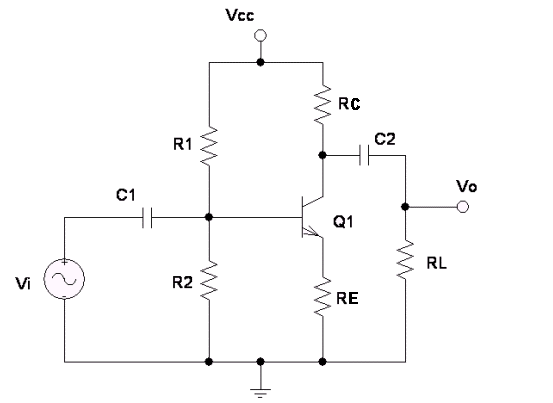
\includegraphics[width = \columnwidth]{imagenes/Circuito.png}
	\caption[Figura3]{Sample of results from bands 1 and 8 from the Verilog version of the filter bank, compared against data from the BeagleBoard's filter version.}
	\label{fig:FiguraCircuito}
\end{figure}


\section{IMÁGENES A COLOR}
Esta permitido el uso de imágenes a color.

Las citas, referencias y ecuaciones deberán de seguir los siguientes criterios: \cite{stat}

\subsection{ECUACIONES}

Por favor utilice símbolos que estén disponibles en  inglés y en español, en las versiones de procesadores de textos.

Las ecuaciones deberán estar numeradas con el número entre paréntesis y al margen derecho del texto, Ej.

\begin{equation} 
\label{eq:evaluacion_iniciatialization}
H=G\left(\frac{b_{01}+b_{11}z^{-1}}{a_{01}+a_{11}z^{-1}} \right)\left(\frac{b_{02}+b_{12}z^{-1}+b_{22}z^{-1}}{a_{02}+a_{12}z^{-1}+a_{22}z^{-1}} \right)
\end{equation}


Para su mención utilice la abreviatura Ec.~\ref{eq:evaluacion_iniciatialization}, a menos que se mencione al inicio de la oración. 

\textbf{Si desea insertar el simbolo de Ohm utilice el comando:}

\begin{verbatim}
    $\Omega$
\end{verbatim}





\section{CITAS Y/O REFERENCIAS}

Las citas y/o referencias se colocarán al final del manuscrito. Para ayudar a los lectores, evite notas a pie de página que incluyen las observaciones periféricas necesarias en el texto (dentro de paréntesis, si usted prefiere, como en esta oración). Las citas deberán de respetar el orden de aparición en las referencias.

Se colocarán entre corchetes Ej. \cite{stat1}. El punto final de la oración se coloca después de la referencia. Para realizar esto, utilice el comando de Latex:

\begin{verbatim}
    \cite{NOMBRE_CITA}
\end{verbatim}

Si es preciso mencionar los nombres de los autores deberán de aparecer todos los nombres exceptuando si el numero de éstos es más de cuatro, en tal caso se pondrá el nombre del primer autor y la leyenda ‘et al’.


% trigger a \newpage just before the given reference
% number - used to balance the columns on the last page
% adjust value as needed - may need to be readjusted if
% the document is modified later
%\IEEEtriggeratref{8}
% The "triggered" command can be changed if desired:
%\IEEEtriggercmd{\enlargethispage{-5in}}

% references section

% can use a bibliography generated by BibTeX as a .bbl file
% BibTeX documentation can be easily obtained at:
% http://www.ctan.org/tex-archive/biblio/bibtex/contrib/doc/
% The IEEEtran BibTeX style support page is at:
% http://www.michaelshell.org/tex/ieeetran/bibtex/
%\bibliographystyle{IEEEtran}
% argument is your BibTeX string definitions and bibliography database(s)
%\bibliography{IEEEabrv,../bib/paper}
%
% <OR> manually copy in the resultant .bbl file
% set second argument of \begin to the number of references
% (used to reserve space for the reference number labels box)
\nocite{*}
\renewcommand{\refname}{Bibliografia}
\bibliographystyle{unsrt}
\bibliography{test}

% biography section
% 
% If you have an EPS/PDF photo (graphicx package needed) extra braces are
% needed around the contents of the optional argument to biography to prevent
% the LaTeX parser from getting confused when it sees the complicated
% \includegraphics command within an optional argument. (You could create
% your own custom macro containing the \includegraphics command to make things
% simpler here.)
%\begin{IEEEbiography}[{\includegraphics[width=1in,height=1.25in,clip,keepaspectratio]{mshell}}]{Michael Shell}
% or if you just want to reserve a space for a photo:

%\begin{IEEEbiography}{Michael Shell}
%Biography text here.
%\end{IEEEbiography}

% if you will not have a photo at all:
%\begin{IEEEbiographynophoto}{John Doe}
%Biography text here.
%\end{IEEEbiographynophoto}

% insert where needed to balance the two columns on the last page with
% biographies
%\newpage

%\begin{IEEEbiographynophoto}{Jane Doe}
%Biography text here.
%\end{IEEEbiographynophoto}

% You can push biographies down or up by placing
% a \vfill before or after them. The appropriate
% use of \vfill depends on what kind of text is
% on the last page and whether or not the columns
% are being equalized.

%\vfill

% Can be used to pull up biographies so that the bottom of the last one
% is flush with the other column.
%\enlargethispage{-5in}



% that's all folks
\end{document}


